\chapter{Data}

We use a corpus of Bach chorales provided by \texttt{music21}. The chorales are
arranged by the Bach-Werke-Verzeichnis (BWV) numbering system, which is one of
the best known and widely used catalogues of Bach's compositions.

Each chorale has four parts and are structured such that the melody is in
the Soprano part and the remaining parts harmonize the melody.

\section{Preprocessing}

\begin{figure}[htbp]
    \centering
    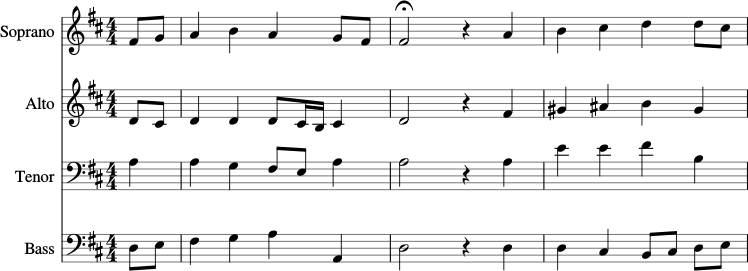
\includegraphics[width=1.0\linewidth]{Figures/bwv133-6-original-score-1.png}
    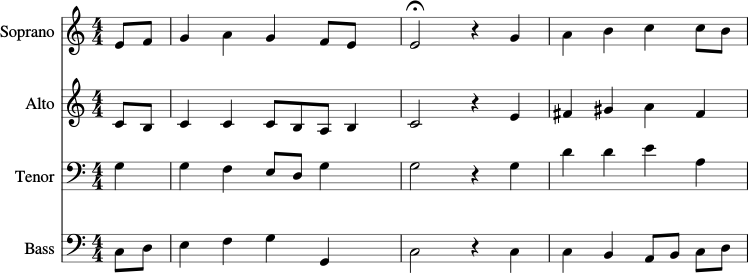
\includegraphics[width=1.0\linewidth]{Figures/bwv133-6-preproc-score-1.png}
    \caption{First 4 bars of JCB Chorale BWV 133.6 before (top) and after (bottom) preprocessing. Note
    the transposition down by a semitone to C-major as well as quantization of the
    semiquavers to quavers in Alto bar 2.}
    \label{fig:score-effects-preproc}
\end{figure}

\begin{figure}[htpb]
    \centering
        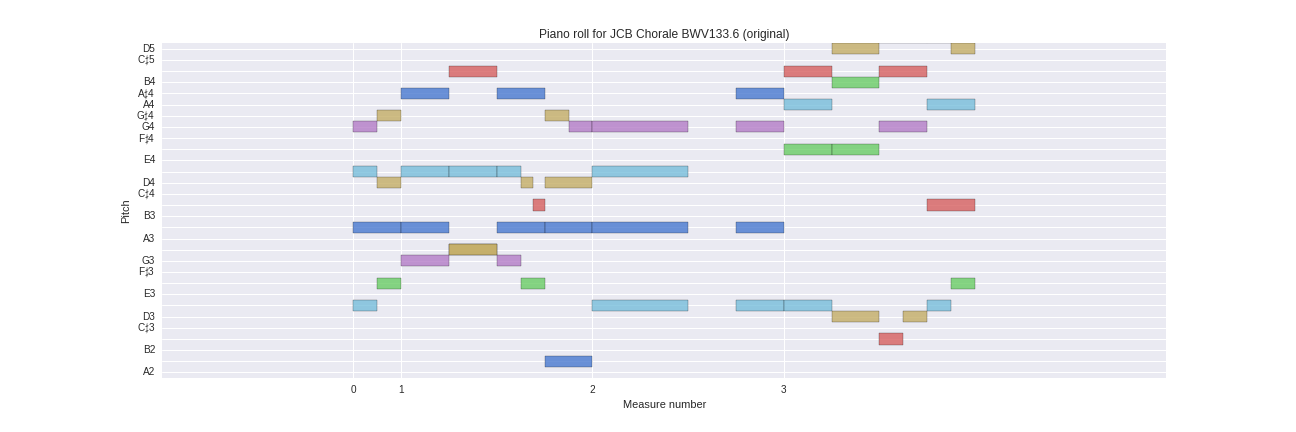
\includegraphics[width=1.0\linewidth]{Figures/bwv133-6-original-piano-roll.png}
        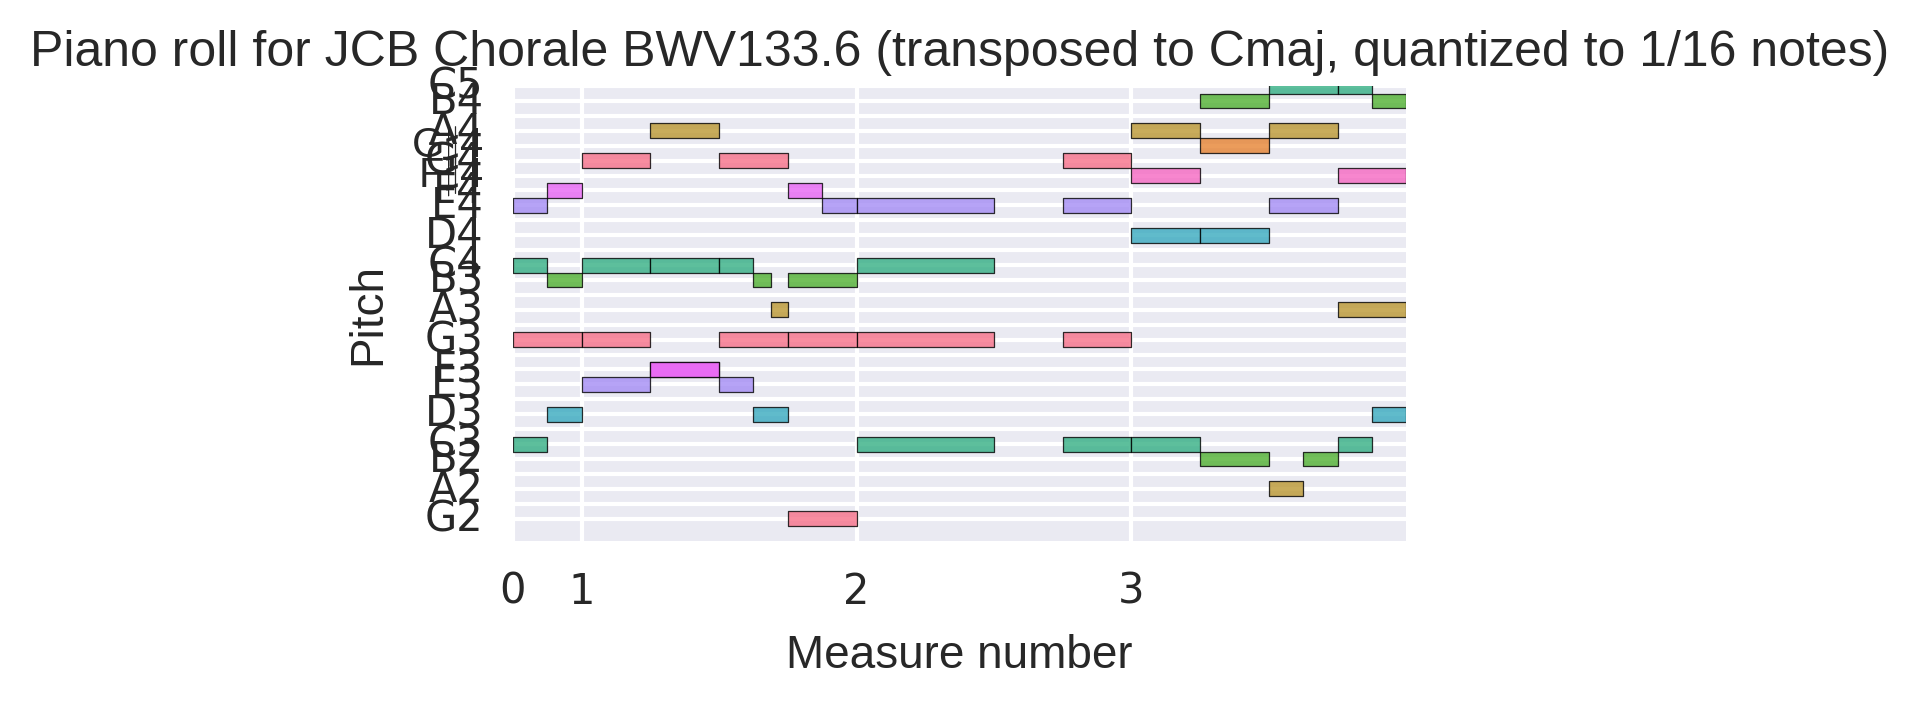
\includegraphics[width=1.0\linewidth]{Figures/bwv133-6-preproc-piano-roll.png}
    \caption{Piano roll representation of the same 4 bars from \autoref{fig:score-effects-preproc}
    before and after preprocessing.}
    \label{fig:piano-roll-effects-preproc}
\end{figure}

\begin{figure}[htpb]
    \centering
    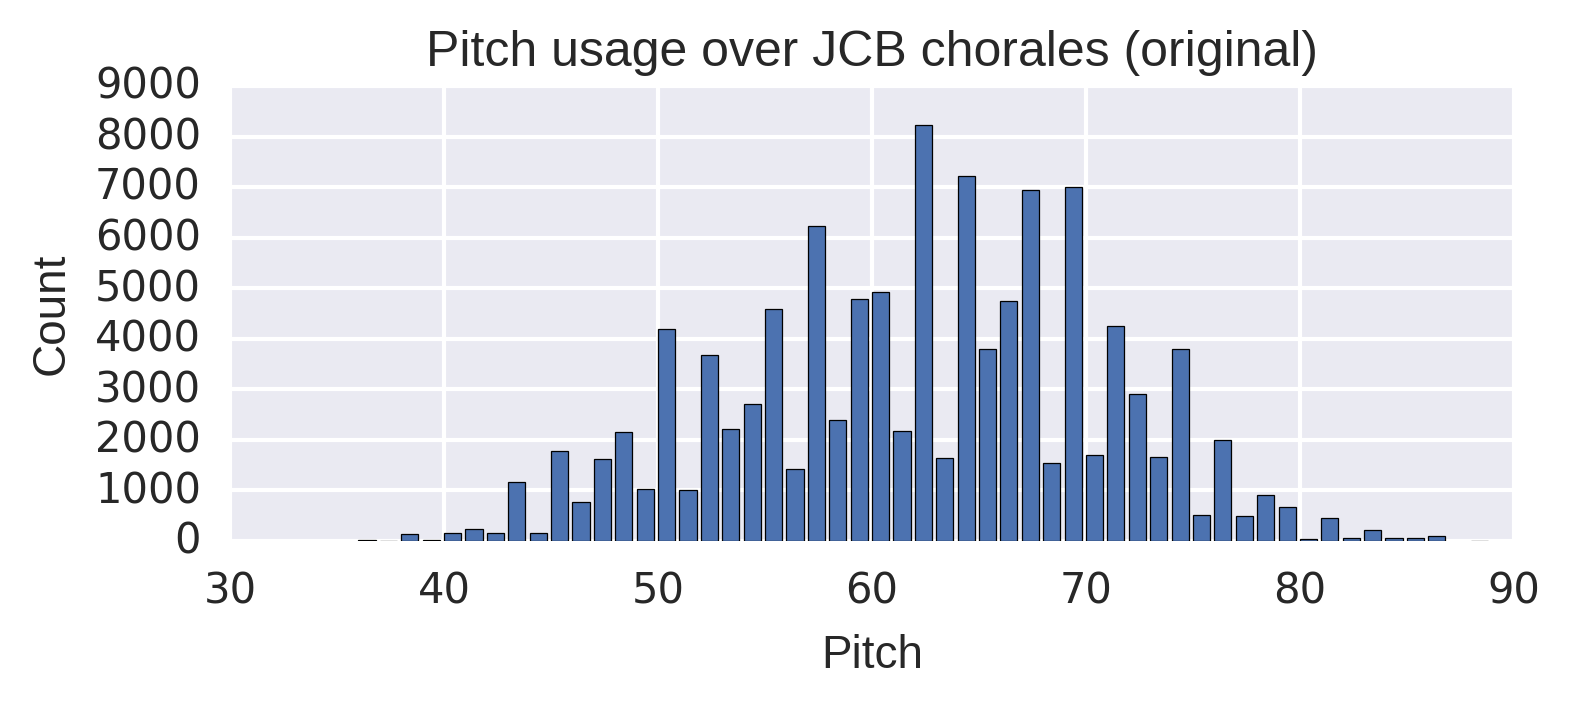
\includegraphics[width=1.0\linewidth]{Figures/pitch-usage-original.png}
    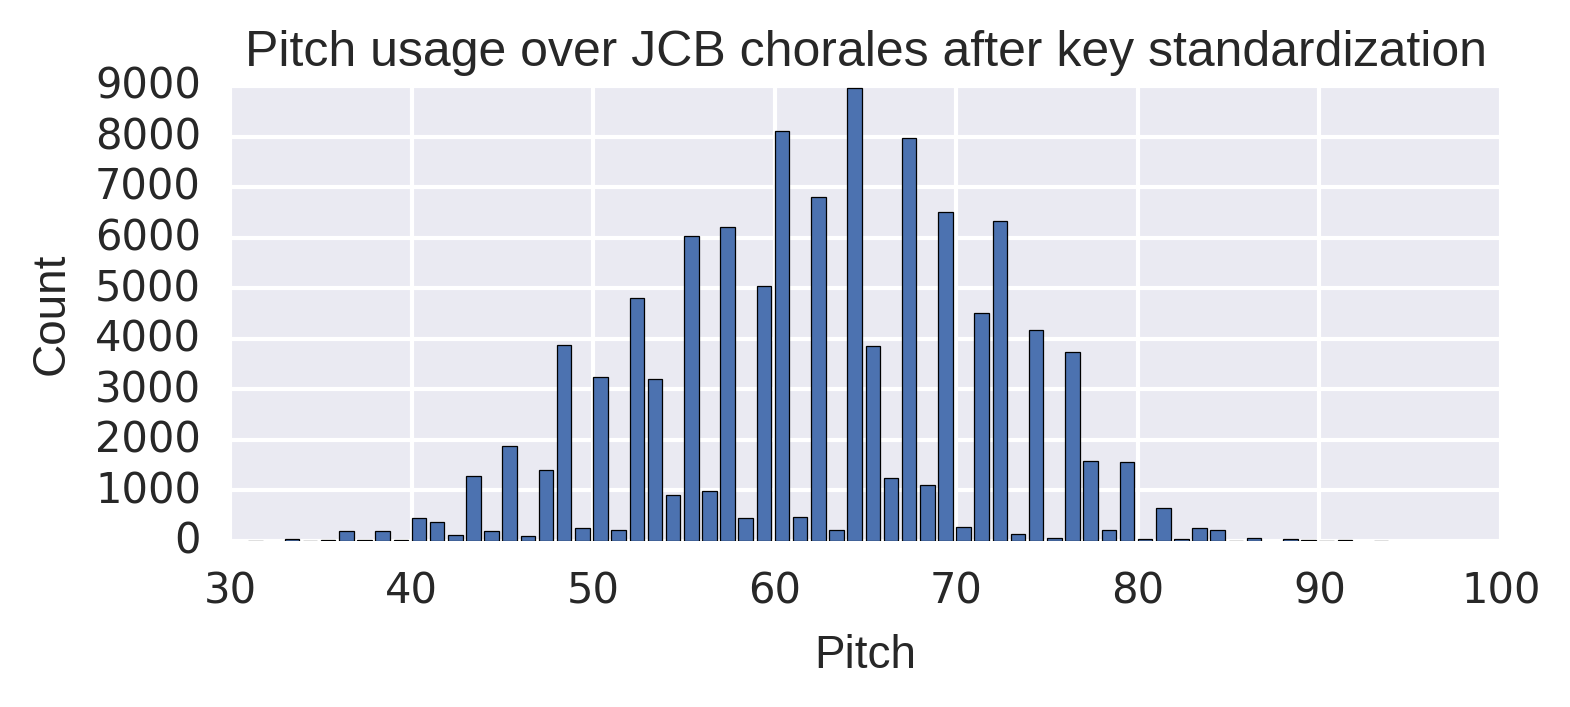
\includegraphics[width=1.0\linewidth]{Figures/pitch-usage-preproc.png}
    \caption{Pitches before and after key standardization}
    \label{fig:pitch-key-standardization}
\end{figure}

\begin{figure}
    \centering
    \begin{subfigure}[b]{0.48\textwidth}
        \centering
        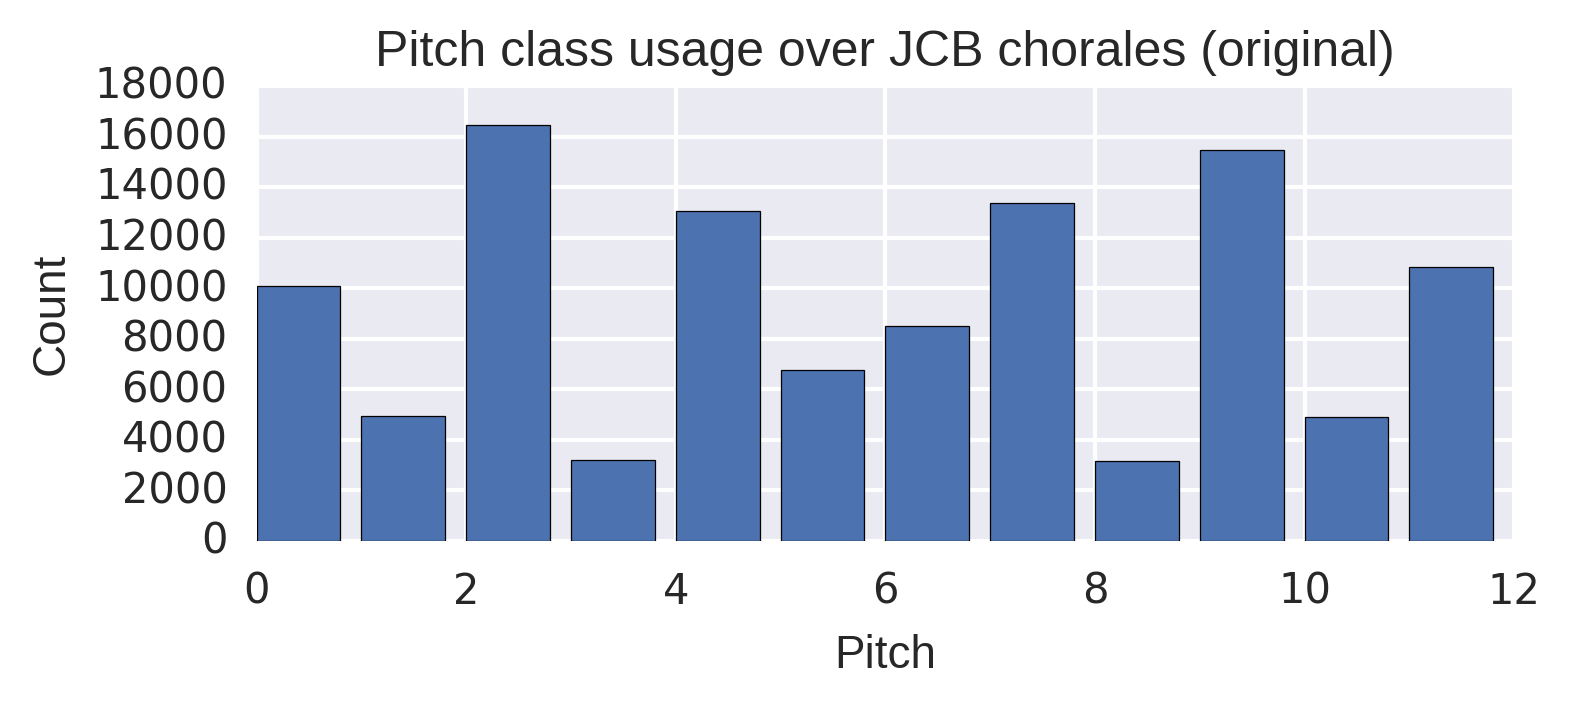
\includegraphics[width=1.0\linewidth]{Figures/pitch-class-usage-original.png}
    \end{subfigure}
    \begin{subfigure}[b]{0.48\textwidth}
        \centering
        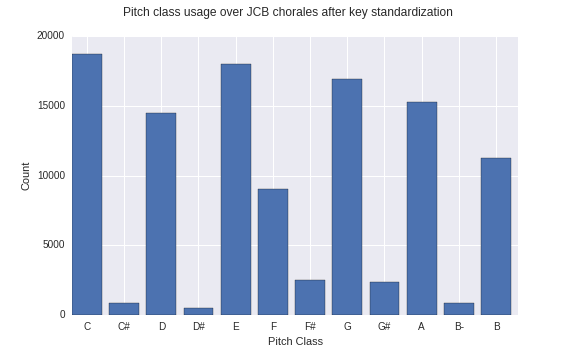
\includegraphics[width=1.0\linewidth]{Figures/pitch-class-usage-preproc.png}
    \end{subfigure}
    \caption{Pitch classes before and after key standardization}
    \label{fig:pc-key-standardization}
\end{figure}

\begin{figure}[htpb]
    \centering
    \begin{subfigure}[t]{0.48\textwidth}
        \centering
        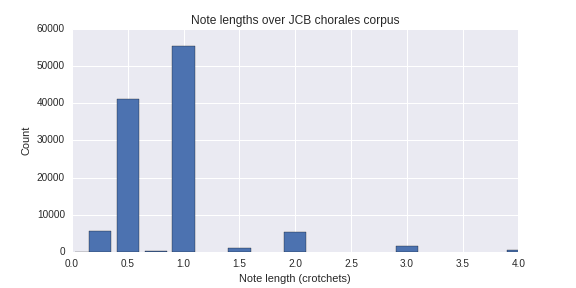
\includegraphics[width=1.0\linewidth]{Figures/note-lengths-original.png}
    \end{subfigure}
    ~
    \begin{subfigure}[t]{0.48\textwidth}
        \centering
        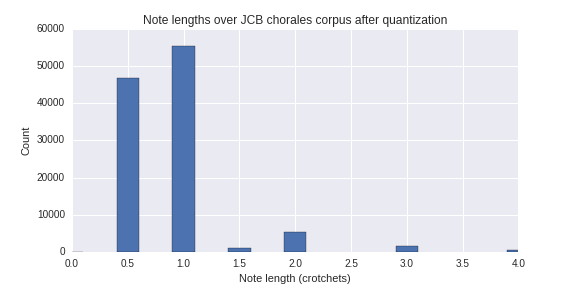
\includegraphics[width=1.0\linewidth]{Figures/note-lengths-quantized.png}
    \end{subfigure}
    \caption{Effects of time quantization on note durations}
    \label{fig:note-lengths-time-quantization}
\end{figure}

\begin{figure}[htpb]
    \centering
    \begin{subfigure}[t]{0.48\textwidth}
        \centering
        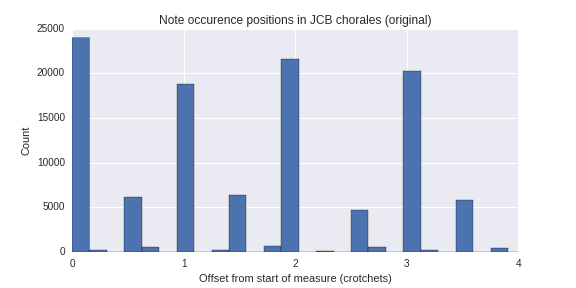
\includegraphics[width=1.0\linewidth]{Figures/meter-usage-original.png}
    \end{subfigure}
    ~
    \begin{subfigure}[t]{0.48\textwidth}
        \centering
        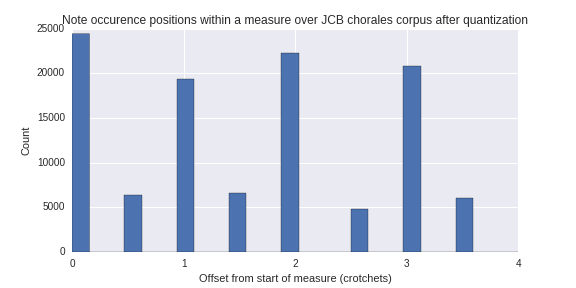
\includegraphics[width=1.0\linewidth]{Figures/meter-usage-quantized.png}
    \end{subfigure}
    \caption{Effects of time quantization on meter}
    \label{fig:meter-time-quantization}
\end{figure}

We represent musical scores using a piano roll representation. Firstly, time is
discretized into constant timestep frames. For each frame, a set of (note, tie)
pairs representing which a note's pitch and whether it is tied
(continuing a note from the previous frame) or newly played notes.


We transpose all scores with major key signatures to C major and minor key
signatures to A minor. Due to transposition invariance of 12-TET, this does
not alter the tonal properties of the music.

\begin{enumerate}
    \item Transpose to Cmaj/Amin
    \item Strip all dynamics info
    \item Restrict to 4/4
\end{enumerate}

Both frame-based processing and quantization to eighth notes justified by Eck
and Smidhuber LSTM Blues \todo{cite}. Eight network time steps are required to
process a whole note. This is preferrable for the LSTM because it forces the network to learn
relative duration of notes, making it easier for counting and timing mechanisms
to be encoded by the LSTM dynamics \todo{Cite Gers and Schmidhuber, 2000}.

\textbf{Contribution}: solved problem of determining when notes end (\todo{cite
Eck Schmidhuber LSTM blues}) in input data format by using the ties.


\subsection{Notation}

We consider note duration, time, and velocity. We neglect changes in timing
(e.g. ritardandos), dynamics (e.g. crescendos), and stylistic notations (e.g.
accents, staccatos, legatos).


\emph{Piano roll} music transcriptions
(\autoref{fig:piano-roll-effects-preproc}) are quantized both in time ($t \in
T$) and note frequencies ($n \in N$). frequencies quantized to a piano roll.
\todo{Motivate quantization with Western music}.

We can represent a piano roll transcription as a high-dimensional vecctor
$X_{t,n} \in \RR^{|T| \times |N|}$ where $X_{t,n}$ denotes the note
velocities for note $n$ at time $t$.

